%% Main manuscript. Layout: style/nature-article.sty; notation: style/macros.sty.
%% Figures in figures/ are generated by simulation/plotting/make_figures.py.
%% Build: latexmk -pdf main.tex   (or pdflatex, bibtex, pdflatex x2)
\documentclass[10pt,twocolumn,a4paper]{article}
\usepackage{style/nature-article}
\usepackage{style/macros}
\graphicspath{{figures/}}

\begin{document}

\twocolumn[{%
\begin{flushleft}
{\sffamily\small Article\par}
\vspace{4pt}
{\sffamily\bfseries\LARGE Radial EIT cooling of lattice-trapped atoms\\[2pt] in a hollow-core fibre with an LP$_{11}$ probe\par}
\vspace{10pt}
{\sffamily\normalsize \note{Author list}\par}
\vspace{2pt}
{\sffamily\footnotesize \note{Affiliations}\quad Draft, \today\par}
\vspace{12pt}
\begin{minipage}{0.86\textwidth}
\bfseries\normalsize
Guided light in a hollow-core fibre propagates along the axis and cannot address the soft radial motion of lattice-trapped atoms. Here we propose radial electromagnetically-induced-transparency (EIT) cooling with the coupling beam in the LP$_{01}$ mode and the probe in the LP$_{11}$ mode, whose node lies on the trap axis. As for an ion at a standing-wave node, the carrier vanishes and the probe couples to the motion only through its gradient. Master-equation simulations for $^{87}$Rb in a \SI{1064}{nm} lattice give, with nanowatts of probe power, cooling rates of $1.3\times10^3$\,s$^{-1}$ ($15\um$ core radius) and $1.2\times10^4$\,s$^{-1}$ ($3.5\um$), with steady-state occupations of 0.13 and 0.04. Cooling from \SI{10}{\micro K} takes about \SI{150}{ms} and \SI{3}{ms}, respectively, and the cooling time grows linearly with the initial temperature up to a tenth of the lattice depth. A simple rate model reproduces the weak-probe limit but overestimates rates and purity tolerance at the optimal working point. The key experimental requirement is an LP$_{11}$ probe with less than $10^{-3}$ LP$_{01}$ power content.
\end{minipage}
\end{flushleft}
\vspace{14pt}
}]

% =====================================================================
% Introduction (unheaded, as in Nature-family articles)
% =====================================================================
Laser-cooled atoms loaded into hollow-core fibres (HCFs) form long, dense ensembles with a strong coupling to a single guided mode\cite{bajcsy2011,blatt2014}. In a one-dimensional lattice formed by the fundamental LP$_{01}$ mode they have enabled Lamb--Dicke spectroscopy\cite{okaba2014} and guided atom interferometry\cite{xin2018}, and the axial motion has been cooled to the ground state by Raman sideband cooling\cite{leong2020}. The radial motion is roughly 40 times softer and remains thermal, because every guided beam propagates along the axis and carries no transverse momentum.

Electromagnetically induced transparency (EIT) cooling uses the Fano profile of a driven $\Lambda$ system to suppress carrier and blue-sideband absorption\cite{morigi2000}. It has cooled trapped ions\cite{roos2000} and neutral atoms\cite{haller2015} to the ground state. Here we show that it can cool the radial motion inside an HCF if the probe is launched in the LP$_{11}$ mode. The LP$_{11}$ field vanishes on the axis and grows linearly with the radial displacement, so the atom sits at a probe node. This is the situation analysed by Cirac \emph{et al.} for an ion in a standing wave\cite{cirac1992}: the carrier disappears and the light couples to the motion through its gradient only.

We first give the principle and a simple rate model, then present master-equation simulations for $^{87}$Rb in two representative fibres and state where the simple model holds. We close with implementations and applications. Derivations and numerical details are given in Methods.

% =====================================================================
\section{Results}
% =====================================================================
\subsection{Gradient coupling at the fibre node}
If probe and coupling beams share the LP$_{01}$ profile, the dark state $\ket D\propto\Om_c\gp-\Om_p\gc$ does not depend on the radial coordinate, and the radial motion is not cooled. We therefore put the probe in LP$_{11}$. In the capillary approximation\cite{marcatili1964,snyder1983} its field is linear near the axis (Fig.~\ref{fig:mechanism}a, Methods):
\begin{equation}
  \Om_p(\hat x)\simeq\bar\Om_p\,G_{11}\frac{\hat x}{a}=\Om_\perp(b+b^\dagger),
  \label{eq:etap}
\end{equation}
with $\Om_\perp=\etap\bar\Om_p$, $\etap=G_{11}x_0/a$ and $G_{11}=3.49$. Here $a$ is the core radius, $x_0=\sqrt{\hbar/2m\omega_r}$, and $\bar\Om_p$ is the Rabi frequency the same power would give at the LP$_{01}$ peak. The probe drives only $\Delta n=\pm1$ and never the carrier. The node is fixed to the axis by symmetry, so it coincides with the lattice centre without alignment. The gradient coupling is small, $\etap\approx0.02$--0.04, but this costs only probe power, because there is no carrier to limit it.

\begin{figure*}[t]
\centering
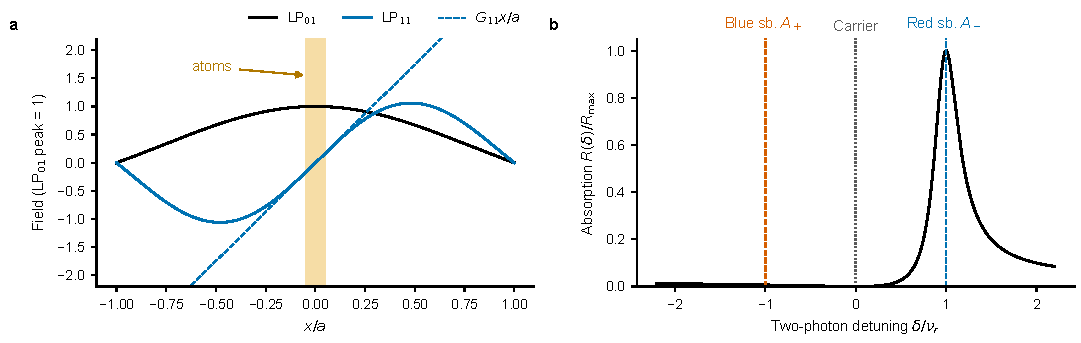
\includegraphics[width=\textwidth]{mechanism.pdf}
\caption{\textbf{Gradient coupling at the fibre node.} \panel{a}, Transverse field profiles at equal guided power for an $a=15\um$ core. The LP$_{11}$ probe has a node on the axis, where the LP$_{01}$ lattice confines the atoms (shaded: thermal extent at \SI{10}{\micro K}). \panel{b}, Weak-probe absorption spectrum, equation~\eqref{eq:fano}, for $\Delta=3\Gamma$ and $\Om_c$ set so that the narrow resonance sits at $\delta=\nu_r$ (case A). sb., sideband.}
\label{fig:mechanism}
\end{figure*}

\begin{figure}[t]
\centering
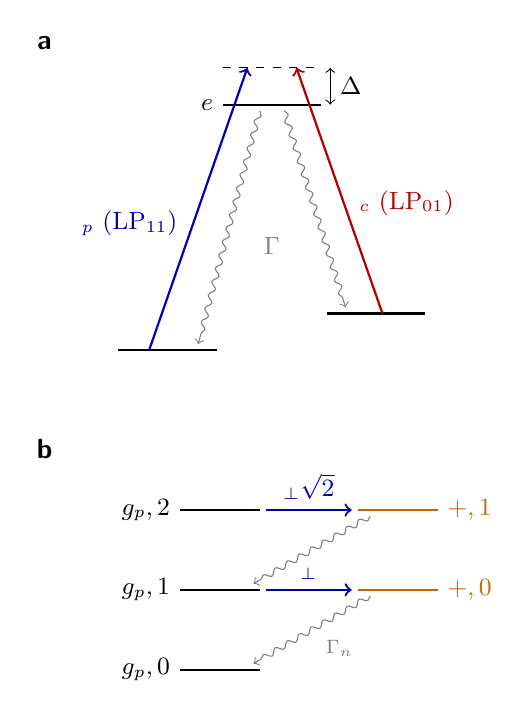
\begin{tikzpicture}[scale=0.78,every node/.style={font=\small},
  wav/.style={->,gray,decorate,decoration={snake,amplitude=1pt,segment length=5pt,post length=3pt}}]
\node[font=\sffamily\bfseries] at (-1.2,5.0) {a};
\draw[thick] (0,0)--(1.6,0) node[below=2pt,midway]{$\gp$};
\draw[thick] (3.4,0.6)--(5.0,0.6) node[below=2pt,midway]{$\gc$};
\draw[thick] (1.7,4.0)--(3.3,4.0);
\node[left] at (1.7,4.0) {$\ket e$};
\draw[dashed] (1.7,4.6)--(3.3,4.6);
\draw[<->] (3.45,4.0)--(3.45,4.6) node[midway,right]{$\Delta$};
\draw[->,thick,blue!70!black] (0.5,0)--(2.1,4.6) node[pos=0.45,left=2pt]{$\Om_p$ (LP$_{11}$)};
\draw[->,thick,red!70!black] (4.3,0.6)--(2.9,4.6) node[pos=0.45,right=2pt]{$\Om_c$ (LP$_{01}$)};
\draw[wav] (2.3,3.9)--(1.3,0.1);
\draw[wav] (2.7,3.9)--(3.7,0.7);
\node[gray] at (2.5,1.7) {$\Gamma$};
\begin{scope}[yshift=-5.2cm,xshift=1.0cm]
\node[font=\sffamily\bfseries] at (-2.2,3.6) {b};
\foreach \n in {0,1,2}{
  \draw[thick] (0,1.3*\n)--(1.3,1.3*\n);
  \node[left] at (0,1.3*\n) {$\ket{g_p,\n}$};
}
\foreach \m in {0,1}{
  \draw[thick,orange!80!black] (2.9,1.3*\m+1.3)--(4.2,1.3*\m+1.3);
  \node[right,orange!80!black] at (4.2,1.3*\m+1.3) {$\ket{+,\m}$};
}
\draw[->,thick,blue!70!black] (1.4,1.3)--(2.8,1.3) node[midway,above]{$\Om_\perp$};
\draw[->,thick,blue!70!black] (1.4,2.6)--(2.8,2.6) node[midway,above]{$\Om_\perp\sqrt2$};
\draw[wav] (3.1,1.2)--(1.2,0.1);
\node[gray,font=\scriptsize] at (2.6,0.35) {$\Gamma_n$};
\draw[wav] (3.1,2.5)--(1.2,1.4);
\end{scope}
\end{tikzpicture}
\caption{\textbf{Cooling scheme.} \panel{a}, $\Lambda$ system on the $^{87}$Rb D1 line. \panel{b}, Dressed picture for $\delta_+=\nu_r$: $\ket{g_p,n}$ and $\ket{+,n-1}$ are degenerate (equal height). The probe gradient drives the resonant red sideband (horizontal arrows); the blue sideband is detuned by $2\nu_r$ and suppressed by the Fano zero; the carrier is not driven.}
\label{fig:levels}
\end{figure}

\subsection{Dressed-state picture and simple rate model}
The coupling beam (detuning $\Delta>0$) dresses $\gc$ into a narrow state $\ket+$ with light shift $\delta_+\simeq\Om_c^2/4\Delta$ and width $\Gamma_n\simeq\Gamma\Om_c^2/4\Delta^2$ (Fig.~\ref{fig:levels}). For $\delta_+=\nu_r$ the probe resonantly drives $\ket{g_p,n}\to\ket{+,n-1}$, and $\ket+$ decays back. The weak-probe absorption spectrum is the Fano profile\cite{morigi2000,fleischhauer2005}
\begin{equation}
  R(\delta)=\frac{\Om_p^2\,\Gamma\,\delta^2}{\Gamma^2\delta^2+4\big[(\Delta+\delta)\delta-\Om_c^2/4\big]^2},
  \label{eq:fano}
\end{equation}
and the sideband rates are $A_\mp=\etap^2R(\pm\nu_r)$ (Fig.~\ref{fig:mechanism}b). Each cycle emits $\kappa=1/b_p\approx2$ photons ($b_p$: branching ratio into $\gp$), each depositing on average $\alpha\eta_{\rm sp}^2$ radial quanta, with $\eta_{\rm sp}=k_{795}x_0$ and $\alpha=2/5$. With the saturation parameter $s=2\Om_\perp^2/\Gamma\Gamma_n$, the simple model\cite{morigi2000} (fibre-specific terms in Methods) gives
\begin{equation}
\begin{aligned}
  W&\simeq(1-h)\frac{\Gamma_n}{2}\frac{s}{1+s},\\
  n_{\rm ss}&\simeq\Big(\frac{\Gamma}{4\Delta}\Big)^2\frac{1+h}{1-h}(1+s),
\end{aligned}
  \label{eq:simple}
\end{equation}
with $h=\kappa\alpha\eta_{\rm sp}^2$. The rate is bounded by the width of the narrow resonance, $\Gamma_n\simeq\Gamma\nu_r/\Delta$, independently of $\etap$. A carrier-present scheme would instead scale as $\etap^2$ (ref.~\citenum{morigi2003}). A residual LP$_{01}$ amplitude $\epsilon$ in the probe restores a carrier; the simple model tolerates $\epsilon\lesssim2.8\,\etap$ (Methods).

\subsection{Two fibre platforms}
We solve the master equation for a $\Lambda$ atom coupled to one radial oscillator, with the exact Bessel mode profiles and spontaneous-emission recoil weighted by the dipole pattern\cite{cirac1992} (Methods). The axial motion is frozen, since co-propagating probe and coupling beams give an axial Lamb--Dicke parameter below $10^{-3}$. Imperfections enter as an LP$_{01}$ admixture $\epsilon$, a trap offset $x_s$ from the node, and a two-photon detuning error $\delta_{\rm e}$. For thermal states with $\langle n\rangle\approx30$ we use a generalised rate model (GRM) calibrated against the master equation. Table~\ref{tab:params} lists the two cases; atomic data are from ref.~\citenum{steck87}.

\begin{table}[t]
\caption{\textbf{Parameters of the two fibre cases.} Lattice \SI{1064}{nm}, $\nu_z=\SI{300}{kHz}$ ($U_0/k_B=\SI{530}{\micro K}$); EIT on the $^{87}$Rb D1 line, $\Gamma/2\pi=\SI{5.75}{MHz}$, $\Delta=3\Gamma$.}
\label{tab:params}
\centering\footnotesize\sffamily
\begin{tabular}{@{}lcc@{}}
\toprule
& A: antiresonant & B: bandgap\\
& $a=15\um$ & $a=3.5\um$\\
\midrule
$\nu_r/2\pi$ & \SI{7.15}{kHz} & \SI{30.6}{kHz}\\
$x_0$; $\etap$ & \SI{90}{nm}; 0.021 & \SI{44}{nm}; 0.043\\
$\eta_{\rm sp}$; $h$ & 0.71; 0.40 & 0.34; 0.094\\
$\Om_c/2\pi$ & \SI{0.70}{MHz} & \SI{1.45}{MHz}\\
$\Gamma_n/2\pi$ & \SI{2.4}{kHz} & \SI{10.2}{kHz}\\
Probe power at $s=1$ & \SI{8}{nW} & \SI{0.4}{nW}\\
$\langle n_x\rangle$ at \SI{10}{\micro K} & 29 & 6.3\\
\bottomrule
\end{tabular}
\end{table}

\subsection{Rate and final occupation}
Figure~\ref{fig:saturation} shows $W$ and $n_{\rm ss}$ versus probe strength. At weak probe the master equation and equation~\eqref{eq:simple} agree within 5\%, provided $\kappa=2$; with $\kappa=1$ the model underestimates $n_{\rm ss}$ by 40\% in case A. The weak-probe floor is $n_{\rm ss}=0.017$ (A) and 0.009 (B). At $s=1$, $W=1.3\times10^3$\,s$^{-1}$ with $n_{\rm ss}=0.13$ (A) and $W=1.2\times10^4$\,s$^{-1}$ with $n_{\rm ss}=0.04$ (B), 25--50 times faster than a carrier-present scheme. The maximum rate, $3.3\times10^3$ and $1.8\times10^4$\,s$^{-1}$, is reached at $s\approx5$ at the cost of $n_{\rm ss}=0.4$ and 0.2.

Above $s\approx0.1$ the simple model overestimates $W$ by up to 65\% and underestimates $n_{\rm ss}$ by up to a factor of 4. Here $s=2(\Om_R/\Gamma_n)^2$, with $\Om_R=\Om_c\Om_\perp/2\Delta$ the Raman coupling between $\ket{g_p,n}$ and $\ket{g_c,n\mp1}$. When $\Om_R$ approaches $\Gamma_n$ the narrow resonance splits, which a perturbative rate picture cannot capture (Methods).

\begin{figure*}[t]
\centering
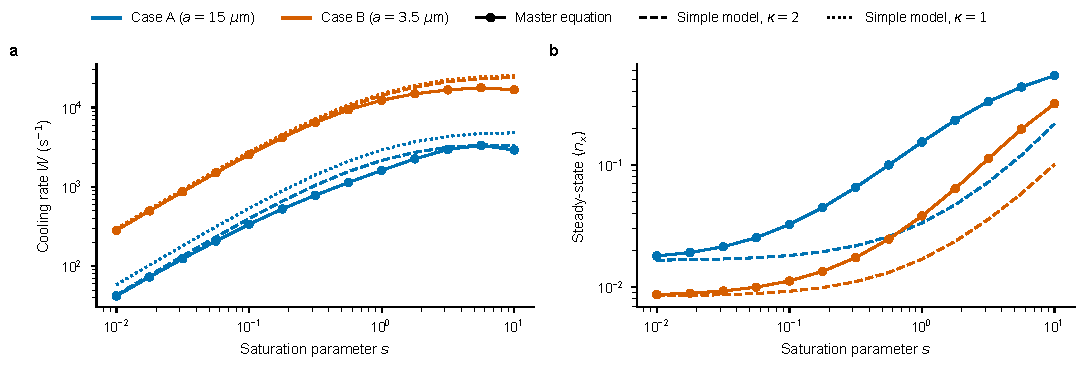
\includegraphics[width=\textwidth]{saturation.pdf}
\caption{\textbf{Cooling rate and final occupation versus probe strength.} \panel{a}, Cooling rate. \panel{b}, Steady-state occupation. $s$ is the saturation parameter of the narrow resonance; $s=1$ corresponds to \SI{8}{nW} (case A) and \SI{0.4}{nW} (case B) of probe power. Symbols, master equation; lines, simple model, equation~\eqref{eq:simple}, with $\kappa$ photons per cycle.}
\label{fig:saturation}
\end{figure*}

\subsection{Robustness}
\paragraph{Mode impurity.} The maximum rate falls gradually with the LP$_{01}$ admixture: by 23\% at $\epsilon=0.01$ and by half at $\epsilon\approx1.4\,\etap\approx0.03$ (Fig.~\ref{fig:robust}a). The simple model's threshold is too optimistic by a factor of two. A trap offset $x_s$ is exactly equivalent to $\epsilon_{\rm eff}=\etap x_s/x_0$.

\paragraph{Two-photon detuning.} With a clean node, a positive error $\delta_{\rm e}$ only reduces the rate (halved at $+0.25\,\nu_r$), while $n_{\rm ss}$ stays below 0.05 up to $+0.6\,\nu_r$ (Fig.~\ref{fig:robust}b). With $\epsilon=0.05$ the carrier heats on both sides. This is the node advantage identified in ref.~\citenum{cirac1992}.

\paragraph{Trap-frequency mismatch.} For fixed lasers, $W$ stays above 70\% of its maximum for $|\nu_r/\nu_r^{\rm design}-1|\lesssim0.1$ (Fig.~\ref{fig:robust}c). This sets the uniformity required along a long strip (Methods).

\begin{figure*}[t]
\centering
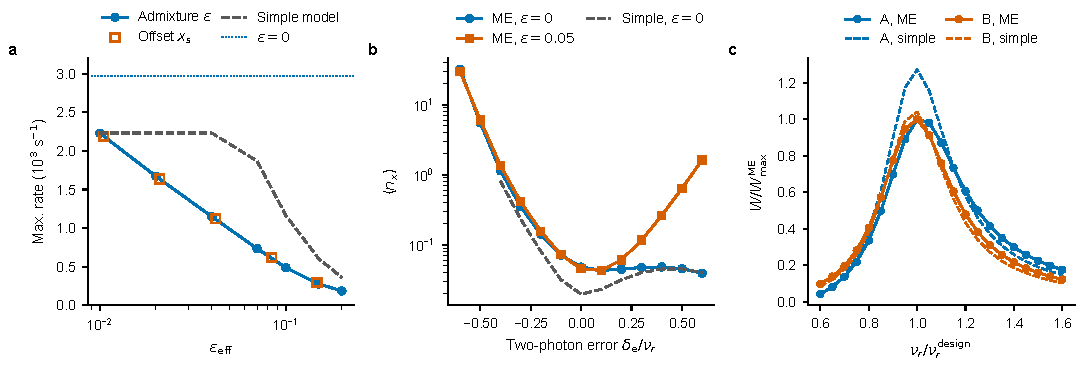
\includegraphics[width=\textwidth]{robust.pdf}
\caption{\textbf{Robustness of radial EIT cooling.} Case A unless stated; ME, master equation. \panel{a}, Maximum rate (optimised over $s\le3$) versus LP$_{01}$ admixture $\epsilon$ and versus trap offset expressed as $\epsilon_{\rm eff}=\etap x_s/x_0$. \panel{b}, Steady-state occupation versus two-photon detuning error at $s=0.2$. \panel{c}, Rate versus actual trap frequency for lasers set for $\nu_r^{\rm design}$, $s=0.2$, both cases.}
\label{fig:robust}
\end{figure*}

\subsection{Cooling dynamics}
The phonon-removal rate per atom saturates at 1.3--1.9 phonons per ms (A) and 10--12 phonons per ms (B). That is only 30--45\% of the naive bound $(1-h)\Gamma_n/2$, because each decay into $\gc$ prolongs the cycle. A GRM calibrated to this saturation reproduces the master-equation dynamics within 8\% (Fig.~\ref{fig:dynamics}a). From \SI{10}{\micro K}, the hot thermal tail dominates in case A: a staged protocol ($\Delta=\Gamma$ for \SI{40}{ms}, then $\Delta=3\Gamma$) brings 97.5\% of the atoms to $n=0$ after \SI{150}{ms}. The mean, $\langle n_x\rangle=1.4$, is still carried by a hot tail of 0.4\% of the atoms with $n\geq20$ (see below). Case B reaches $\langle n_x\rangle=0.04$ in \SI{2.4}{ms} (Fig.~\ref{fig:dynamics}b,c). An LP$_{12}$ probe gives identical curves: in the carrier-free regime the rate depends on $s$, not on the mode order.

\begin{figure*}[t]
\centering
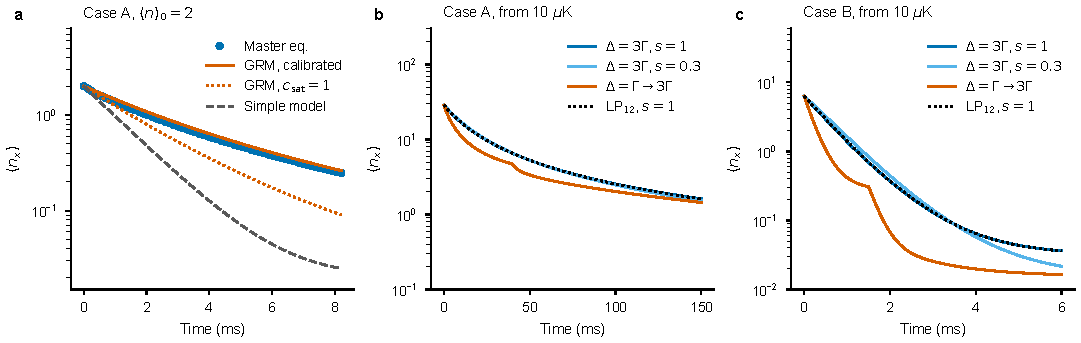
\includegraphics[width=\textwidth]{dynamics.pdf}
\caption{\textbf{Cooling dynamics.} \panel{a}, $\langle n_x\rangle(t)$ for case A at $s=0.2$ from a thermal state with $\langle n\rangle=2$: master equation, generalised rate model (GRM) with and without calibrated saturation, and single-exponential simple model. \panel{b},\panel{c}, Cooling from \SI{10}{\micro K} with the calibrated GRM. The staged protocol switches from $\Delta=\Gamma$, $s=1$ to $\Delta=3\Gamma$, $s=0.3$ at \SI{40}{ms} (case A) and \SI{1.5}{ms} (case B).}
\label{fig:dynamics}
\end{figure*}

\subsection{Dependence on the initial temperature}
To separate the role of temperature from that of the trap, we start from thermal states with $k_BT_r/U_0=10^{-3}$--$10^{-1}$ in 20 logarithmic steps ($T_r=0.5$--\SI{53}{\micro K} for $U_0/k_B=\SI{530}{\micro K}$). Over this range the radial potential is harmonic to within 4\% (anharmonic shift $\approx\tfrac38k_BT_r/U_0$), the atoms stay well inside the core ($x_{\rm th}\lesssim0.11a$) and less than $10^{-4}$ of them lie above the trap depth. At equal $k_BT_r/U_0$ the oscillator of case B is 4.3 times colder, $\bar n_0\simeq(k_BT_r/U_0)\,U_0/\hbar\nu_r$ with $U_0/\hbar\nu_r=1552$ (A) and 362 (B). Figure~\ref{fig:temperature} shows two regimes. For $\bar n_0\lesssim3$ the cooling is close to exponential at the rate $W$. Above, the red sideband saturates, the initial phonon-removal rate approaches a constant, 1.9 (A) and 12 (B) phonons per ms, and the cooling time grows linearly with temperature. The time to bring 90\% of the atoms to $n=0$ is $t_{90}\approx\SI{2.5}{s}\times k_BT_r/U_0$ (A) and $\approx\SI{80}{ms}\times k_BT_r/U_0$ (B), i.e.\ \SI{255}{ms} and \SI{7.7}{ms} at $k_BT_r/U_0=0.1$. The ground state is reached over the whole range. The mean occupation converges more slowly than $P_0$ (Fig.~\ref{fig:temperature}a,b): recoil makes the energy of hot atoms diffuse, so a small fraction is pushed to high $n$ and is cooled only at the saturated rate. A small core thus gains twice at higher temperature: its oscillator is colder for the same $k_BT_r/U_0$, and it removes six times more phonons per unit time.

\begin{figure*}[t]
\centering
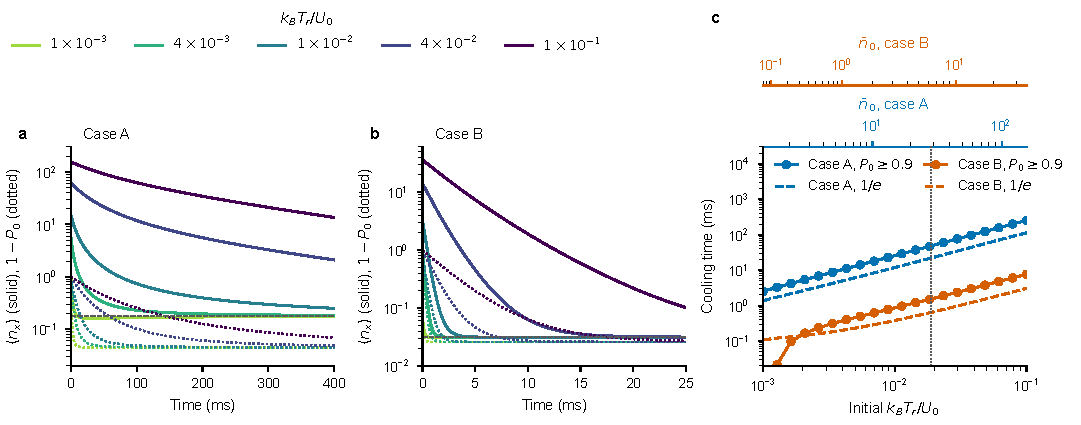
\includegraphics[width=\textwidth]{temperature.pdf}
\caption{\textbf{Cooling versus initial radial temperature.} Calibrated GRM, $\Delta=3\Gamma$, $s=1$, LP$_{11}$ probe, from thermal states with $k_BT_r/U_0=10^{-3}$--$10^{-1}$. \panel{a},\panel{b}, $\langle n_x\rangle(t)$ (solid) and the population outside the ground state $1-P_0$ (dotted) for five initial temperatures; dashed grey, steady state. \panel{c}, Time to reach $P_0\geq0.9$ (circles) and $1/e$ time of the excess $\langle n_x\rangle-n_{\rm ss}$ (dashed). The dotted line marks \SI{10}{\micro K} (Fig.~\ref{fig:dynamics}b,c). Top axis: $T_r$ for $U_0/k_B=\SI{530}{\micro K}$.}
\label{fig:temperature}
\end{figure*}

\subsection{Validity of the simple model}
Table~\ref{tab:validity} summarises the comparison. The simple model captures the mechanism and is quantitative at weak probe, provided it counts $\kappa=1/b_p$ photons per cycle. It is not reliable at the working points that maximise the rate, for the impurity tolerance, or for cooling from a thermal state. Both descriptions neglect the Zeeman structure of the D1 line (which increases $\kappa$ and pushes case A towards $h\to1$), the second radial axis and collective effects.

\begin{table*}[t]
\caption{\textbf{Simple model versus master equation (ME).}}
\label{tab:validity}
\centering\footnotesize\sffamily
\begin{tabular}{@{}p{4.0cm}p{5.0cm}p{7.6cm}@{}}
\toprule
Quantity & Simple model & Master equation\\
\midrule
$n_{\rm ss}$, $W$ at weak probe & equation~\eqref{eq:simple} & within 5\% if $\kappa=2$\\
$W$, $n_{\rm ss}$ at $s\sim1$ & equation~\eqref{eq:simple} & $W$ up to 65\% lower, $n_{\rm ss}$ up to 4$\times$ higher\\
Mode impurity & $\epsilon\lesssim2.8\,\etap$ & rate halved at $\epsilon\approx1.4\,\etap$\\
Two-photon error & sideband shift on Fano profile & agrees where $W>0$\\
Trap-frequency mismatch & Fano profile & shape within 20--30\%\\
Cooling from \SI{10}{\micro K} & single exponential & too fast; saturated removal rate is 30--45\% of the bound\\
\bottomrule
\end{tabular}
\end{table*}

% =====================================================================
\section{Discussion}
% =====================================================================
\paragraph{Experimental challenges.}
(i) \emph{Probe purity}: the LP$_{01}$ power content must stay below $10^{-3}$, preferably $10^{-4}$. It can be measured by spatially and spectrally resolved imaging\cite{nicholson2008}. Fibres that suppress higher-order modes\cite{uebel2016,poletti2014} clean the lattice beam but also attenuate LP$_{11}$; the allowed differential loss is $\approx\SI{9}{dB}$ for a launch purity $\epsilon_0=0.01$ (Methods).
(ii) \emph{Vector modes}: TE$_{01}$, TM$_{01}$ and HE$_{21}$ beat and rotate the lobe pattern and polarisation along the fibre\cite{ramachandran2013}. The node stays on axis, but polarisation variation opens the $\Lambda$ system.
(iii) \emph{Multilevel atom and light shifts}: leakage out of the $\Lambda$ system increases $\kappa$. The lattice's differential light shift ($\approx\SI{0.8}{kHz}$)\cite{kuhr2005} lies within the detuning window of Fig.~\ref{fig:robust}b once compensated.
(iv) \emph{Uniformity along the strip}: the coupling power must vary by less than $\approx\SI{0.8}{dB}$ across the strip; the lattice loss is not limiting (Methods).
(v) \emph{Technical heating}: lattice intensity and pointing noise heat the radial motion directly\cite{savard1997}.
(vi) \emph{Axial cooling}: one Fano peak cannot serve both $\nu_r$ and $\nu_z\approx40\nu_r$. Radial EIT and axial sideband cooling\cite{leong2020} must be alternated, or a double-EIT scheme used\cite{scharnhorst2018}.
The radial temperature can be read out by Raman sideband spectroscopy\cite{kerman2000} with one LP$_{11}$ and one LP$_{01}$ beam.

\paragraph{Implementation I: large-core antiresonant fibre.} A nested antiresonant fibre with $2a\approx\SI{30}{\micro m}$, low loss at both 795 and \SI{1064}{nm}\cite{sakr2020}, is mounted vertically and loaded from a magneto-optical trap above its tip\cite{bajcsy2011}. The LP$_{11}$ probe is generated with a spatial light modulator\cite{flamm2013}, combined with the LP$_{01}$ coupling beam and launched from the same end. Expected performance (case A): 2--\SI{8}{nW} of probe power, $W\approx10^3$\,s$^{-1}$ and 97\% of the atoms in $n=0$ after \SI{150}{ms}. This is the more mature option; its weakness is the slow capture of the thermal tail.

\paragraph{Implementation II: small-core fibre section.} A 1--\SI{5}{cm} piece of photonic-bandgap fibre with $2a\approx\SI{7}{\micro m}$ is loaded by a moving lattice\cite{okaba2014}. The probe is injected from the nearer end so that the lossy LP$_{11}$ mode, which can be excited selectively in HCF\cite{trabold2014}, travels only a few cm. Cooling is ten times faster (ground state in \SI{3}{ms}) and the recoil per cycle is four times smaller. The costs are a smaller loading volume, stronger modal loss and the proximity of the core wall.

\paragraph{Applications.} Combined with axial sideband cooling\cite{leong2020}, the scheme would give centimetre-long strips of three-dimensionally ground-state-cooled atoms inside a single-mode waveguide.
(i) \emph{Long-lived spin-wave quantum memories}: in lattice memories, motional dephasing and the thermally averaged differential light shift limit the storage time\cite{zhao2009,dudin2013}. Radial ground-state cooling reduces the thermal broadening from $\approx\SI{15}{Hz}$ at \SI{10}{\micro K} to $\sim\SI{0.01}{Hz}$ (Methods), and the large optical depth of a fibre strip allows efficient storage\cite{gorshkov2007}, beyond current HCF memories with free-falling atoms\cite{peters2020}.
(ii) \emph{Waveguide quantum electrodynamics and atomic Bragg mirrors}\cite{corzo2016,chang2018}: a smaller radial spread reduces coupling inhomogeneity and disorder.
(iii) \emph{Guided atom interferometry}\cite{xin2018} and \emph{lattice clocks}\cite{okaba2014}: reduced transverse dephasing and light-shift inhomogeneity.
(iv) \emph{Rydberg nonlinear optics}\cite{langbecker2017}: less motional dephasing, and atoms further from the core wall.

\paragraph{Conclusion.} An LP$_{11}$ probe turns the fibre geometry into a carrier-free node configuration for radial EIT cooling. For an ideal $\Lambda$ system, master-equation simulations predict rates of $10^3$--$10^4$\,s$^{-1}$ and occupations of 0.02--0.2 with nanowatts of probe power. Small cores are strongly favoured, because they raise $\nu_r$ and lower the recoil per cycle. The decisive experimental requirement is an LP$_{11}$ probe purity of $\lesssim10^{-3}$. The simple rate model is a good design tool at weak probe but must be replaced by the master equation, or a calibrated rate model, at the optimal working point. Next steps are simulations with the full D1 Zeeman structure and both radial axes.

% =====================================================================
\section{Methods}
% =====================================================================
\paragraph{Mode profiles and trap parameters.}
In the capillary model the LP$_{lm}$ modes are $\psi_{lm}=A_{lm}J_l(u_{lm}r/a)\cos l\phi$ with $J_l(u_{lm})=0$, so $u_{01}=2.405$ and $u_{11}=3.832$ (refs.~\citenum{marcatili1964,snyder1983}). Equal guided power, $\int|\psi|^2dA$, gives $A_{01}^2\pi a^2J_1^2(u_{01})=A_{11}^2\tfrac{\pi a^2}{2}J_2^2(u_{11})$, hence
\begin{equation}
  \frac{A_{11}}{A_{01}}=\frac{\sqrt2\,|J_1(u_{01})|}{|J_2(u_{11})|}=1.82 .
\end{equation}
With $J_1(z)\simeq z/2$, the LP$_{11}$ field near the axis is $A_{01}G_{11}x/a$ with $G_{11}=(u_{11}/2)A_{11}/A_{01}=3.49$, which gives equation~\eqref{eq:etap}. The LP$_{01}$ intensity is close to a Gaussian with waist $w=0.67a$ (best fit to $J_0^2$). A standing wave of depth $U_0$ and wavenumber $k_L$ then gives
\begin{equation}
  \omega_z=\sqrt{\frac{2U_0k_L^2}{m}},\quad \omega_r=\sqrt{\frac{4U_0}{mw^2}},\quad \frac{\omega_z}{\omega_r}=\frac{k_Lw}{\sqrt2},
\end{equation}
i.e.\ $\nu_r=\SI{7.15}{kHz}$ ($a=15\um$) and \SI{30.6}{kHz} ($a=3.5\um$) for $\nu_z=\SI{300}{kHz}$ at \SI{1064}{nm}. The probe power corresponding to $\bar\Om_p$ is $P=2I_{\rm sat}(\bar\Om_p/\Gamma)^2\pi a^2J_1^2(u_{01})$, with $I_{\rm sat}=\SI{4.48}{mW\,cm^{-2}}$ (ref.~\citenum{steck87}). The axial wavevector difference between LP$_{11}$ and LP$_{01}$, $(u_{11}^2-u_{01}^2)/2ka^2$, is \SI{2.5}{mm^{-1}} (A) and \SI{46}{mm^{-1}} (B), giving axial Lamb--Dicke parameters below $10^{-3}$.

\paragraph{Simple-model terms specific to the fibre.}
The Fano profile, the sideband rates and the rate equation follow Morigi \emph{et al.}\cite{morigi2000}, with $\Om_c^2=4\nu_r(\Delta+\nu_r)$ placing the narrow resonance on the red sideband. Three additions enter equation~\eqref{eq:simple}. (i) After a decay into $\gc$ (probability $1-b_p$) the coupling beam re-excites the atom, so a cycle emits $\kappa=1/b_p$ photons, each depositing on average $\alpha\eta_{\rm sp}^2$ radial quanta, exactly for any $\eta_{\rm sp}$; this gives $h=\kappa\alpha\eta_{\rm sp}^2$. (ii) Saturation reduces only the resonant red sideband, $A_-\to A_-/(1+s)$, which gives the factor $(1+s)$ in $n_{\rm ss}$. (iii) An LP$_{01}$ admixture $\epsilon$ gives a carrier $\epsilon\bar\Om_p$; requiring $\epsilon\bar\Om_p\le\Om_c/3$ (ref.~\citenum{morigi2003}) at $s=1$ yields $\epsilon\le(2\sqrt2\Delta/3\Gamma)\etap=2.8\,\etap$ for $\Delta=3\Gamma$. The same condition on a carrier-present probe gives $W\simeq(4\Delta/9\Gamma)\etap^2\nu_r$, about \SI{26}{s^{-1}} (A) and \SI{490}{s^{-1}} (B).

\paragraph{Master equation.}
In the frame rotating at the laser frequencies,
\begin{equation}
\begin{aligned}
  H/\hbar={}&\nu_r b^\dagger b-\Delta\ket e\bra e-\delta_{\rm e}\gc\bra{g_c}\\
  &+\tfrac{\bar\Om_p}{2}\big[f_p(\hat x)\ket e\bra{g_p}+{\rm h.c.}\big]\\
  &+\tfrac{\Om_c}{2}\big[f_c(\hat x)\ket e\bra{g_c}+{\rm h.c.}\big],
\end{aligned}
\end{equation}
\begin{equation}
\begin{aligned}
  \dot\rho&=-\tfrac i\hbar[H,\rho]+\sum_{j=p,c}\sum_k\mathcal D[L_{jk}]\rho,\\
  L_{jk}&=\sqrt{\Gamma b_jw_k}\,\ket{g_j}\bra e\,e^{i\eta_{\rm sp}u_k(b+b^\dagger)},
\end{aligned}
\end{equation}
with $f_p(x)=(A_{11}/A_{01})J_1(u_{11}(x+x_s)/a)+\epsilon J_0(u_{01}(x+x_s)/a)$ and $f_c(x)=J_0(u_{01}(x+x_s)/a)$. The recoil is discretised with ten equal-weight nodes $u_k$ of the distribution of $u_x=\sin\theta\cos\phi$ for a dipole along $z$ ($\langle u_x^2\rangle=0.397$)\cite{cirac1992}; $b_p=b_c=1/2$. Functions of $\hat x$ are evaluated in the eigenbasis of the truncated position operator. Twenty Fock states suffice for $\langle n\rangle\lesssim0.5$ (checked with 30 and 40). The steady state is obtained from $\mathcal L\rho=0$ with the trace condition, using a sparse LU factorisation. The cooling rate is the inverse integrated relaxation time after preparing $\rho_0=\ket{g_p,1}\bra{g_p,1}$,
\begin{equation}
  W^{-1}=\int_0^\infty\!\frac{\langle n\rangle(t)-n_{\rm ss}}{1-n_{\rm ss}}dt=-\frac{{\rm Tr}[\hat n\,\mathcal L^{-1}(\rho_0-\rho_{\rm ss})]}{1-n_{\rm ss}},
\end{equation}
which reuses the same factorisation and, unlike the slowest Liouvillian eigenvalue, is not affected by slow modes at the truncation edge. Time evolution uses a fixed-step BDF2 scheme with $\Delta t=0.02/\nu_r$.

\paragraph{Strong-probe regime.}
The effective Raman coupling between $\ket{g_p,n}$ and $\ket{g_c,n\mp1}$ is $\Om_R=\Om_c\Om_\perp/2\Delta$. With $\Gamma_n\simeq\Gamma\Om_c^2/4\Delta^2$ one finds $\Om_R^2=s\Gamma_n^2/2$. For $s\gtrsim0.1$ the narrow resonance is therefore split and broadened, and a coherent $\gc$ admixture builds up (2.4\% at $s=1$, case A). The off-resonant blue-sideband Raman process then grows faster than $(1+s)$.

\paragraph{Generalised rate model.}
The GRM evolves the populations $p_n$ of $\ket{g_p,n}$ with the rate matrix $Q=TK-{\rm diag}(\sum_mK_{mn})$. The absorption rates
\begin{equation}
  K_{mn}=\frac{\bar\Om_p^2\,|\bra m f_p(\hat x)\ket n|^2\,R\big((n-m)\nu_r\big)/\Om_p^2}{1+c_{\rm sat}s_n}
\end{equation}
include the full Bessel profile; $s_n=s\,|\bra{n-1}\hat x\ket n|^2/x_0^2$ is the saturation of the $n\to n-1$ sideband. The redistribution after absorption is $T=b_pP(1-b_cP)^{-1}$, where $P_{n'm}=\sum_kw_k|\bra{n'}e^{i\eta_{\rm sp}u_k(b+b^\dagger)}\ket m|^2$ is the recoil kernel of one photon. With $c_{\rm sat}=1$ the GRM overestimates the saturated phonon-removal rate by a factor of 2--2.5 (Table~\ref{tab:calib}). Fitting $c_{\rm sat}$ to the master-equation drift $d\langle n\rangle/dt$ from Fock states $n_0=1$--15 at $s=0.2$ and 1, in both cases, gives $c_{\rm sat}=2.25$ with 17\% rms deviation. Thermal dynamics use Fock spaces that extend to the trap depth, $N=1600$ (A) and 400 (B) ($U_0/\hbar\nu_r=1552$ and 362). A smaller truncation is not sufficient in case A: recoil spreads the energy of a hot atom by $\approx\eta_{\rm sp}\sqrt n$ quanta per photon, and a small fraction of atoms diffuses to $n\gtrsim300$, where a truncated Fock space acts as an artificial sink. With $N=300$, $\langle n_x\rangle$ after \SI{150}{ms} (staged, from \SI{10}{\micro K}) would be 0.24 instead of 1.45, while $P_0$ changes by only 0.3\%. Case B is converged at $N=120$. Beyond the calibration range the GRM underestimates the master-equation drift (Table~\ref{tab:calib}): at $s=1$ it gives 0.75 and 0.42 of the master-equation drift for $n_0=20$ and 30 in case A, and 0.83 and 0.56 in case B (master equation with $N=45$ and 60; $N=60$ changes the $n_0=20$ value by 0.3\%). The GRM cooling times of hot thermal states are therefore conservative.

\begin{table}[t]
\caption{\textbf{Calibration of the generalised rate model.} Phonon-removal rate $-d\langle n\rangle/dt$ (ms$^{-1}$) from Fock state $n_0$, case A, $s=1$. The fit uses $n_0\leq15$; $n_0=20$ and 30 test the extrapolation.}
\label{tab:calib}
\centering\footnotesize\sffamily
\begin{tabular}{@{}lccccccc@{}}
\toprule
$n_0$ & 1 & 3 & 6 & 10 & 15 & 20 & 30\\
\midrule
Master equation & 1.20 & 1.49 & 1.35 & 1.41 & 1.86 & 2.55 & 4.57\\
GRM, $c_{\rm sat}=1$ & 2.16 & 3.28 & 3.75 & 3.99 & 4.11 & -- & --\\
GRM, $c_{\rm sat}=2.25$ & 1.33 & 1.69 & 1.81 & 1.87 & 1.89 & 1.91 & 1.92\\
\bottomrule
\end{tabular}
\end{table}

\paragraph{Experimental estimates.}
\emph{Probe purity along the fibre.} The LP$_{01}$ admixture grows as $\epsilon(z)=\epsilon_0e^{(\alpha_{11}-\alpha_{01})z/2}$. Requiring $\epsilon\le1.4\,\etap$ (rate halved) gives a differential-loss budget $(\alpha_{11}-\alpha_{01})L\lesssim20\log_{10}(1.4\etap/\epsilon_0)$\,dB: 9\,dB for $\epsilon_0=0.01$ and 20\,dB for $\epsilon_0=0.003$ (case A).
\emph{Uniformity along the strip.} For counter-propagating lattice beams with power loss $\alpha_L$, the antinode field is $\propto e^{-\alpha_Lz/2}+e^{-\alpha_L(L-z)/2}\propto\cosh[\alpha_L(z-L/2)/2]$, so $\nu_r\propto\cosh[\alpha_L(z-L/2)/2]$; a 10\% variation corresponds to $\approx\SI{8}{dB}$ of lattice loss across the strip. The Fano peak scales as $\delta_+\propto P_c$, so a $\pm10\%$ tolerance limits the coupling-beam loss across the strip to $\approx\SI{0.8}{dB}$.
\emph{Light shifts.} The differential light shift of the hyperfine $\Lambda$ in the \SI{1064}{nm} lattice is $\delta_{\rm diff}\approx U_0\omega_{\rm hfs}/\Delta_{\rm eff}\approx\SI{0.8}{kHz}$ for $U_0/h=\SI{11}{MHz}$ (ref.~\citenum{kuhr2005}). The $F'=1$/$F'=2$ splitting (\SI{814}{MHz}) adds a shift of $\gc$ of order $\Om_c^2/(4\times\SI{814}{MHz})\approx\SI{0.15}{kHz}$, small compared with $\Gamma_n$.
\emph{Other heating and offsets.} Photon scattering from the lattice adds $\sim1$ radial quantum per second. Gravity sag in a horizontal fibre, $g/\omega_r^2=\SI{4.9}{nm}=0.05\,x_0$ (A), corresponds to $\epsilon_{\rm eff}=0.001$.
\emph{Probe depletion.} With $10^5$ atoms each scattering at most $\Gamma_n/2$, the absorbed probe power is $\le\SI{0.2}{nW}$ (A) and $\le\SI{0.8}{nW}$ (B): negligible in case A but comparable to the probe power in case B.
\emph{Memory dephasing.} The thermal spread of the differential light shift is $\delta_{\rm diff}\langle V_\perp\rangle/U_0$, with $V_\perp$ the radial potential energy: $\approx\SI{15}{Hz}$ at \SI{10}{\micro K} and $\sim\SI{0.01}{Hz}$ for $\langle n_x\rangle=\langle n_y\rangle=0.02$ (the zero-point part is common to all atoms).

% =====================================================================
\section{Data availability}
The data generated in this study are provided with the manuscript. \note{repository and DOI}

\section{Code availability}
The simulation and plotting code (Python) is provided with the manuscript. \note{repository and DOI}

{\small
\bibliographystyle{naturemag}
\bibliography{refs}
}

\section{Acknowledgements}
\note{Acknowledgements and funding}

\section{Author contributions}
\note{Author contributions}

\section{Competing interests}
The authors declare no competing interests. \note{to be confirmed}

\end{document}
